\documentclass[a4paper]{article}

\usepackage{a4wide}
\usepackage{tikz}
\usepackage{tikz-qtree}
\usepackage{amsmath,amssymb}

%\usetikzlibrary{automata,positioning,arrows,shapes,matrix}
\usetikzlibrary{automata}    % Styles 'state', 'initial', 'accepting'
\usetikzlibrary{positioning} % Function "of" (e.g. [right=of x])
\usetikzlibrary{backgrounds} % Predefined "background" layer

% TikZ variables
\def\myvdist{1.2cm}
\def\myhdist{0.5cm}

% Colours of components (-1, 1, and 2)  
\newcommand{\x}[1]{\widehat{#1}}
\newcommand{\one}[1]{\overline{#1}}
\newcommand{\two}[1]{\overline{\overline{#1}}}

% Global tikz settings
\tikzset{
semithick, % All lines semithick
>=stealth, % All arrows with stealth tick
my node/.style={minimum height=1.75em,minimum width=2em,inner sep=1mm},
my state/.style={draw,my node,rectangle,rounded corners=2mm},
my accepting/.style={double,double distance=1pt,outer sep=0.9pt,semithick},
longer1/.style={shorten >=-0.425mm,shorten <=-0.5mm},
longer2/.style={shorten >=-0.7mm,shorten <=-0.8mm},
automaton/.style={
  every state/.style={my state},
  accepting/.style={my accepting},
  initial text=,
  every loop/.style={min distance=6mm,looseness=7},
  my below/.style={out=295,in=245},
  my above/.style={out=65,in=115},
  node distance=1cm
},
states/.style={
  every node/.style={my node},
  st/.style={draw,my state},
  acc/.style={my accepting},
},
tree/.style={
  states,
  level distance=\myvdist,
  sibling distance=\myhdist,
},
tree example sets/.style={
  0/.style= {st,font={$\{q_0\}$}},
  1/.style= {st,acc,font={$\{q_1\}$}},
  2/.style= {st,font={$\{q_2\}$}},
  02/.style={st,font={$\{q_0,q_2\}$}},
},
tree example no sets/.style={
  0/.style={st,font={$q_0$}},
  1/.style={st,acc,font={$q_1$}},
  2/.style={st,font={$q_2$}},
},
mtrx/.style={
  states,
  row sep={\myvdist,between origins},
  inner sep=0mm
},
dag/.style={
  mtrx,
  ghost/.style={draw=black!20,color=black!20},
  column sep=0.75cm
}
}

\newcommand{\automaton}{
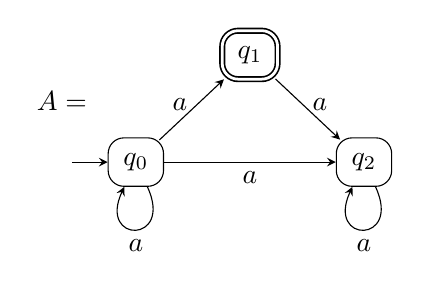
\begin{tikzpicture}[automaton]
\node[state,initial]   (0)                    {$q_0$};
\node[state,accepting] (1) [above right=of 0] {$q_1$};
\node[state]           (2) [below right=of 1] {$q_2$};

\path[->] (0) edge[my below,loop] node[below] {$a$} ()
              edge[longer1]        node[pos=0.3,above](m) {$a$} (1)
              edge                node[below] {$a$} (2)
          (1) edge[longer1]        node[pos=0.7,above] {$a$} (2)
          (2) edge[my below,loop] node[below] {$a$} ();

\node[draw=none,anchor=base,xshift=-1.5cm] at (m.base){$A=$};  
\end{tikzpicture}
}

\newcommand{\symbols}{
\begin{tikzpicture}[
level distance=\myvdist,
l/.style={pos=0.3,font={$a$}},
e/.style={draw=none}]
\Tree [ \edge[e] node[l]{}; [ \edge[e] node[l]{}; [ \edge[e] node[l]{}; [ \edge[e] node[l]{}; {} ] ] ] ]
\end{tikzpicture}
}

\begin{document}

%==============================================================================%
% Split tree
%==============================================================================%
\begin{figure}
\begin{center}
\automaton
\hfill
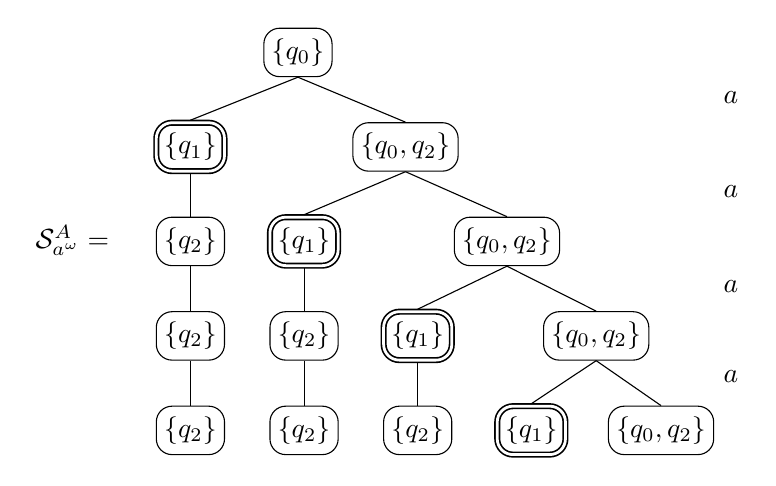
\begin{tikzpicture}[tree,tree example sets]
\Tree
[.\node[0]{}; [.\node[1]{};  [.\node[2](m){};  [.\node[2]{};  \node[2]{}; ] ] ]
              [.\node[02]{}; [.\node[1]{};  [.\node[2]{};  \node[2]{}; ] ]
                             [.\node[02]{}; [.\node[1]{};  \node[2]{}; ]
                                            [.\node[02]{}; \node[1]{};
                                                           \node[02]{}; ] ] ] ]
\node[draw=none,anchor=base,xshift=-1.5cm] at (m.base) {$\mathcal{S}^A_{a^\omega}=$};
\begin{scope}[every node/.style={draw=none,xshift=2.75cm}]
\Tree
[ \edge[draw=none] node[pos=.4]{$a$}; [ \edge[draw=none] node[pos=.4]{$a$}; [ \edge[draw=none] node[pos=.4]{$a$}; [ \edge[draw=none] node[pos=.4]{$a$}; {} ]  ] ] ]
\end{scope}
\end{tikzpicture}
%\symbols
\end{center}
\caption{Automaton $A$ and the first five levels of the split tree of the runs of $A$ on the word $a^\omega$.}
\end{figure}

%==============================================================================%
% Reduced split tree left-to-right
%==============================================================================%
\begin{figure}
\begin{center}
\automaton
\hfill
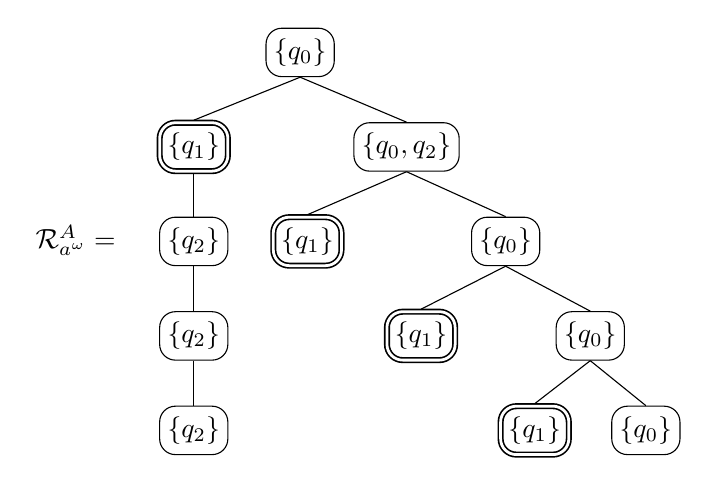
\begin{tikzpicture}[tree,tree example sets]
\Tree
[.\node[0]{}; [.\node[1]{};  [.\node[2](m){}; [.\node[2]{}; \node[2]{}; ] ] ]
              [.\node[02]{};   \node[1]{};
                             [.\node[0]{};      \node[1]{};
                                              [.\node[0]{}; \node[1]{};
                                                            \node[0]{}; ] ] ] ]
\node[draw=none,anchor=base,xshift=-1.5cm] at (m.base) {$\mathcal{R}^A_{a^\omega}=$};
% \begin{scope}[every node/.style={draw=none,xshift=2.75cm}]
% \Tree
% [ \edge[draw=none] node[pos=.4]{$a$}; [ \edge[draw=none] node[pos=.4]{$a$}; [ \edge[draw=none] node[pos=.4]{$a$}; [ \edge[draw=none] node[pos=.4]{$a$}; {} ]  ] ] ]
% \end{scope}
\end{tikzpicture}
\symbols
\end{center}
\caption{Automaton $A$ and the first five levels of the left-to-right reduced split tree of the runs of $A$ on the word $a^\omega$.}
\end{figure}

%==============================================================================%
% Reduced split tree right-to-left
%==============================================================================%
\begin{figure}
\begin{center}
\automaton
\hfill
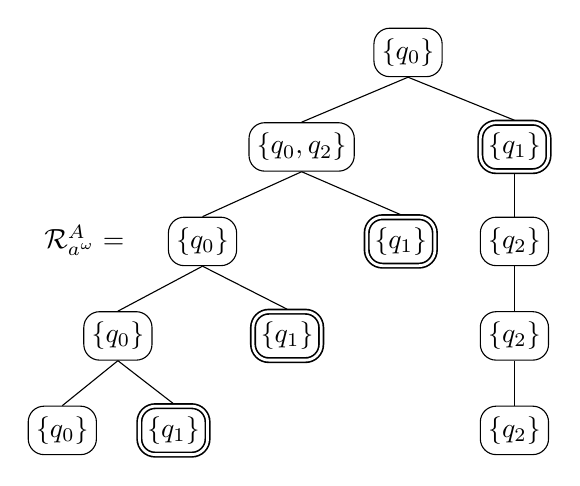
\begin{tikzpicture}[tree,tree example sets]
\Tree
[.\node[0]{}; [.\node[02]{}; [.\node[0](m){}; [.\node[0]{}; \node[0]{};
                                                            \node[1]{}; ] 
                                                \node[1]{}; ]
                               \node[1]{}; ]
              [.\node[1]{};  [.\node[2]{};    [.\node[2]{}; \node[2]{}; ] ] ] ]
\node[draw=none,anchor=base,xshift=-1.5cm] at (m.base) {$\mathcal{R}^A_{a^\omega}=$};
\end{tikzpicture}
\symbols
\end{center}
\caption{Automaton $A$ and the first five levels of the right-to-left reduced split tree of the runs of $A$ on the word $a^\omega$.}
\end{figure}


%==============================================================================%
% Run tree
%==============================================================================%
\begin{figure}
\begin{center}

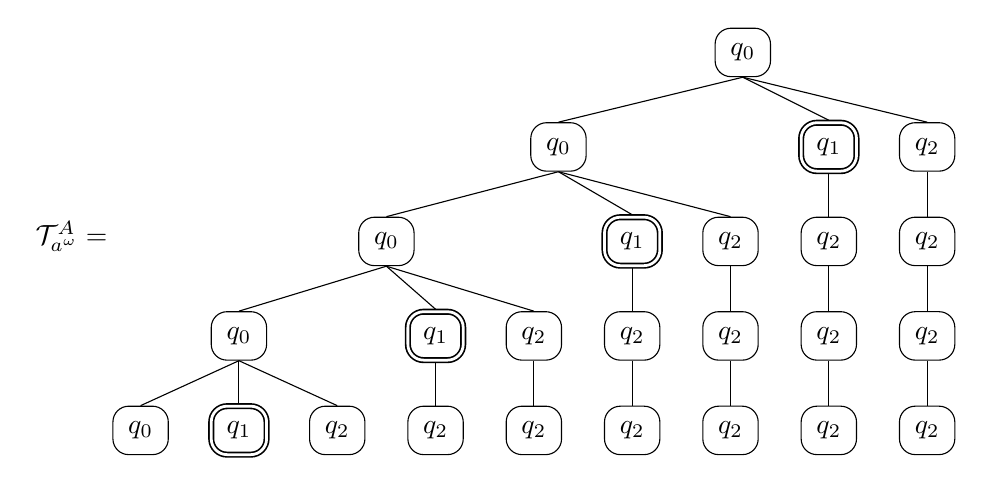
\begin{tikzpicture}[tree,tree example no sets]
\Tree
[.\node[0]{}; [.\node[0]{}; [.\node[0](m){}; [.\node[0]{};  \node[0]{};
                                                            \node[1]{};
                                                            \node[2]{}; ]
                                              [.\node[1]{}; \node[2]{}; ]
                                              [.\node[2]{}; \node[2]{}; ] ]
                            [.\node[1]{};     [.\node[2]{}; \node[2]{}; ] ]
                            [.\node[2]{};     [.\node[2]{}; \node[2]{}; ] ] ]
              [.\node[1]{}; [.\node[2]{};    [.\node[2]{};  \node[2]{}; ] ] ]
              [.\node[2]{}; [.\node[2]{};   [.\node[2]{};  \node[2]{}; ] ] ] ]

\node[draw=none,anchor=base,xshift=-4cm] at (m.base) {$\mathcal{T}^A_{a^\omega}=$};
% \begin{scope}[every node/.style={draw=none,xshift=2.75cm}]
% \Tree
% [ \edge[draw=none] node[pos=.4]{$a$}; [ \edge[draw=none] node[pos=.4]{$a$}; [ \edge[draw=none] node[pos=.4]{$a$}; [ \edge[draw=none] node[pos=.4]{$a$}; {} ]  ] ] ]
% \end{scope}
\end{tikzpicture}
\symbols
\end{center}
\caption{Automaton $A$ and the first five levels of the run tree of the runs of $A$ on the word $a^\omega$.}
\end{figure}


%==============================================================================%
% Run DAG
%==============================================================================%
\begin{figure}
\begin{center}
\automaton
\hfil
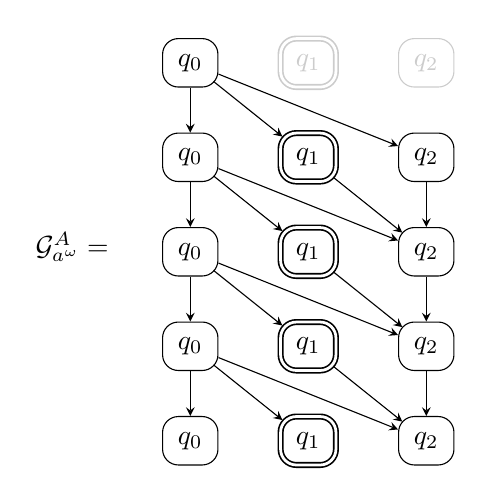
\begin{tikzpicture}[dag,tree example no sets]  
\matrix{
  \node[0] (00) {}; & \node[1,ghost] (01) {}; & \node[2,ghost] (02) {}; \\
  \node[0] (10) {}; & \node[1] (11) {}; & \node[2] (12) {}; \\
  \node[0] (20) {}; & \node[1] (21) {}; & \node[2] (22) {}; \\
  \node[0] (30) {}; & \node[1] (31) {}; & \node[2] (32) {}; \\
  \node[0] (40) {}; & \node[1] (41) {}; & \node[2] (42) {}; \\
};
\path[->]
  (00) edge (10) edge[longer2] (11) edge (12)
  (10) edge (20) edge[longer2] (21) edge (22)
  (11) edge[longer2] (22)
  (12) edge (22)
  (20) edge (30) edge[longer2] (31) edge (32)
  (21) edge[longer2] (32)
  (22) edge (32)
  (30) edge (40) edge[longer2] (41) edge (42)
  (31) edge[longer2] (42)
  (32) edge (42);  
\node[anchor=base,xshift=-1.5cm] at (20.base) {$\mathcal{G}^A_{a^\omega}=$};      
\end{tikzpicture}
\symbols
\end{center}
\caption{Automaton $A$ and the first five levels of the run \textsc{dag} of the runs of $A$ on the word $a^\omega$.}
\end{figure}


%==============================================================================%
% From reduced split tree to subset-tuple slices
%==============================================================================%
\begin{figure}
\begin{center}
\symbols
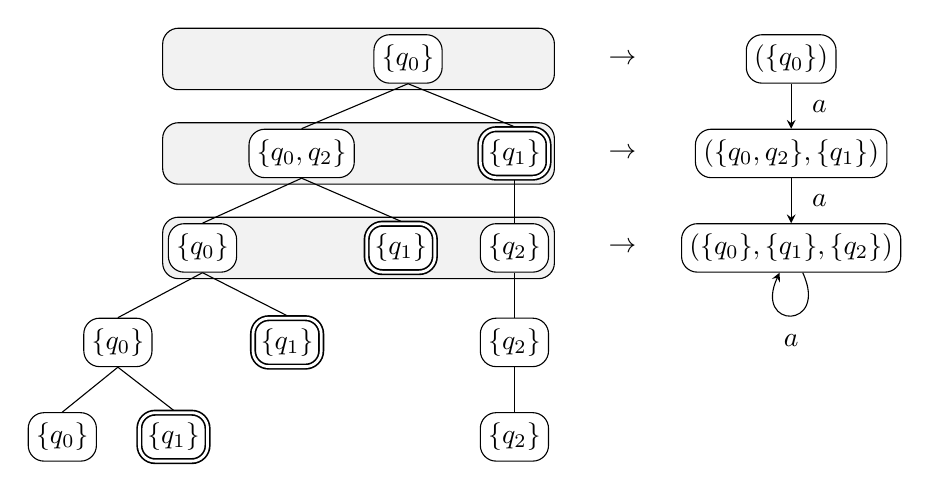
\begin{tikzpicture}[tree,tree example sets,frame/.style={my state,minimum width=4.975cm,minimum height=2.22em,fill=black!5},w/.style={my state,fill=white}]
\Tree
[.\node[w]{$\{q_0\}$}; [.\node[w]{$\{q_0,q_2\}$}; [.\node[w](m){$\{q_0\}$}; [.\node[0]{}; \node[0]{};
                                                            \node[1]{}; ] 
                                                \node[1]{}; ]
                               \node[acc,w]{$\{q_1\}$}; ]
              [.\node[acc,w](a){$\{q_1\}$};  [.\node[w]{$\{q_2\}$};    [.\node[2]{}; \node[2]{}; ] ] ] ]
\begin{scope}[on background layer]
\node[frame,anchor=east,xshift=0.5mm] (m) at (a.east) {};
\node[frame,anchor=center,yshift=\myvdist] (h) at (m.center) {};
\node[frame,anchor=center,yshift=-\myvdist] (l) at (m.center) {};
\end{scope}
\begin{scope}[arrow/.style={xshift=0.5cm,anchor=west}]
\node[arrow] at (h.east) {$\rightarrow$};
\node[arrow] at (m.east) {$\rightarrow$};
\node[arrow] at (l.east) {$\rightarrow$};
\end{scope}
\begin{scope}[slice/.style={my state,xshift=3cm},automaton]
\node[slice] (s1) at (h.east) {$\left(\{q_0\}\right)$};
\node[slice] (s2) at (m.east) {$\left(\{q_0,q_2\},\{q_1\}\right)$};
\node[slice] (s3) at (l.east) {$\left(\{q_0\},\{q_1\},\{q_2\}\right)$};
\path[->] (s1) edge node[right] {$a$} (s2)
          (s2) edge node[right] {$a$} (s3)
          (s3) edge[my below,loop] node[below] {$a$} ();
\end{scope}
\end{tikzpicture}
\end{center}
\caption{From levels of a reduced split tree to the slices of the subset-tuple construction.}
\end{figure}

%==============================================================================%
% Upper part of complement of A
%==============================================================================%
\begin{figure}
\begin{center}
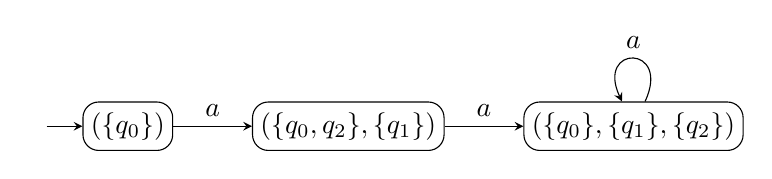
\begin{tikzpicture}[automaton]
\node[state,initial] (0) {$\left(\{q_0\}\right)$};
\node[state]         (1) [right=of 0] {$\left(\{q_0,q_2\},\{q_1\}\right)$};
\node[state]         (2) [right=of 1] {$\left(\{q_0\},\{q_1\},\{q_2\}\right)$};
\path[->] (0) edge node[above]{$a$} (1)
          (1) edge node[above]{$a$} (2)
          (2) edge[my above,loop] node[above]{$a$} ();
\end{tikzpicture}
\end{center}
\caption{Upper part of complement of $A$.}
\end{figure}

%==============================================================================%
% Complement of A
%==============================================================================%
\begin{figure}
\begin{center}
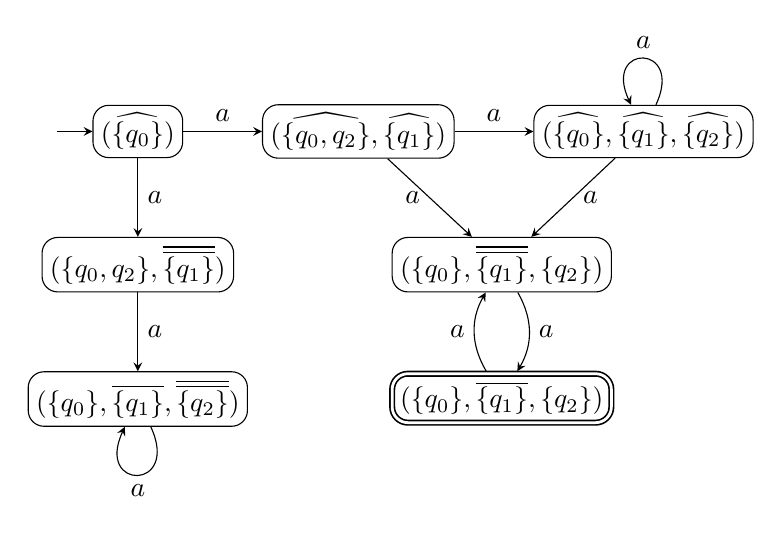
\begin{tikzpicture}[automaton]
\node[state,initial] (0) {$(\x{\{q_0\}})$};
\node[state]         (1) [right=of 0] {$(\x{\{q_0,q_2\}},\x{\{q_1\}})$};
\node[state]         (2) [right=of 1] {$(\x{\{q_0\}},\x{\{q_1\}},\x{\{q_2\}})$};
\node[state]         (01) [below=of 0] {$(\{q_0,q_2\},\two{\{q_1\}})$};
\node[state]         (02) [below=of 01] {$(\{q_0\},\one{\{q_1\}},\two{\{q_2\}})$};
\node[state,xshift=1cm] (11) [right=of 01] {$(\{q_0\},\two{\{q_1\}},\{q_2\})$};
\node[state,accepting]  (12) [below=of 11] {$(\{q_0\},\one{\{q_1\}},\{q_2\})$};
\path[->] (0)  edge                node[above]{$a$} (1)
          (1)  edge                node[above]{$a$} (2)
          (2)  edge[my above,loop] node[above]{$a$} ()
          (0)  edge                node[right]{$a$} (01)
          (01) edge                node[right]{$a$} (02)
          (02) edge[my below,loop] node[below]{$a$} ()
          (1)  edge                node[left] {$a$} (11)
          (11) edge[bend left]     node[right]{$a$} (12)
          (12) edge[bend left]     node[left] {$a$} (11)
          (2)  edge                node[right]{$a$} (11);
\end{tikzpicture}
\end{center}
\caption{The complement automaton $B$.}
\end{figure}


\end{document}